\section[System Struktur (Christopher Althaus)]{System Struktur\begin{tiny} (Christopher Althaus)\end{tiny}}
Die Erdbebenerkennung soll über ein verteiltes System erfolgen. Prinzipiell handelt es sich hierbei um ein Client-Server-System, wobei die Android Smartphones die Clients darstellen. Den Teil des Servers soll ein WebService übernehmen. Die die Strukturierung und Kommunikationsbeziehung dieser beiden Komponenten ist in Abbildung \ref{fig:SystemStrukutr} dargestellt.
\begin{figure}[H]
\centering
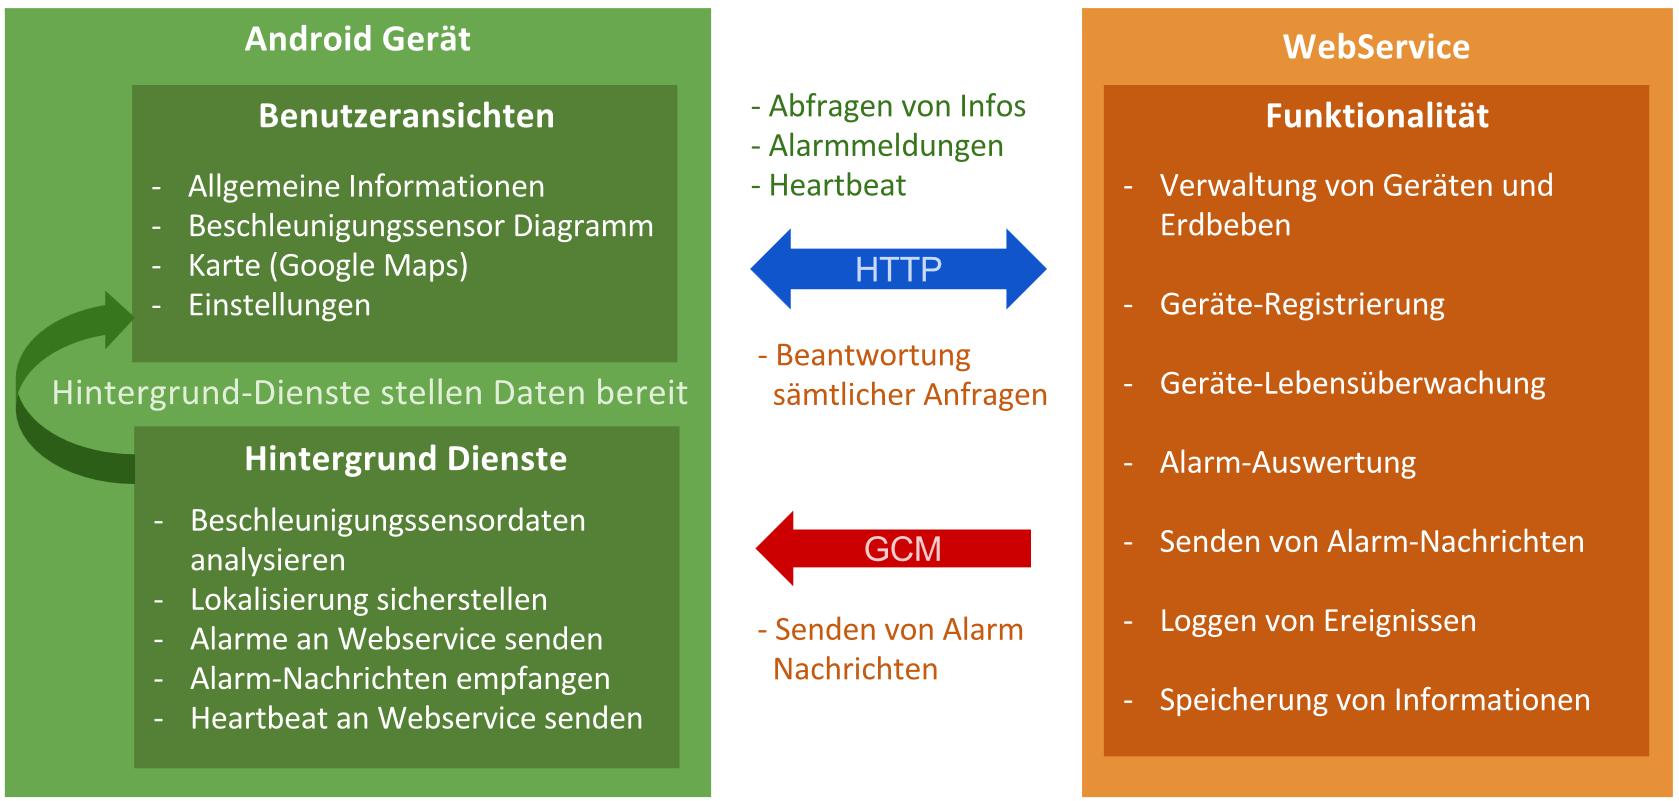
\includegraphics[width=\textwidth]{/Systemstruktur.png}
\caption{Struktur des Projektes}
\label{fig:SystemStrukutr}
\end{figure}
Das rechts dargestellte Android Gerät kann grundlegend in die Benutzeransichten und Hintergrunddienste unterteilt werden.\\
Die Benutzeransichten stellen dabei den für den Nutzer der App sichtbaren Teil dar. Hierzu gehören zum einen allgemeine Informationen, wie das letzte erkannte Erdbeben oder die Anzahl der verbundenen Geräte. Weiterhin soll dem Nutzer ein Diagramm angezeigt werden, welches die Daten des Beschleunigungssensors anzeigt, um dem Benutzer ersichtlich zu machen, dass die Sensorauswertung funktioniert. Ebenso soll innerhalb der Applikation eine Karte angezeigt werden, welche die verbundenen Geräte und die erkannten Erdbeben für den Nutzer visuell darstellt.\\
Um die Applikation für den Nutzer anpassbar zu machen, soll ein Einstellungsmenü existieren, in dem beispielsweise die Alarmeinstellungen geändert werden können.\\
Neben diesen sichtbaren Anteilen bedarf es zahlreicher Hintergrundaktivitäten, welche die eigentlichen Aufgaben der Applikation bewerkstelligen. Zu den wohl Wichtigsten zählen hier die Lokalisierung des Gerätes und die Auswertung der Beschleunigungssensordaten. Diese Dienste sollen beim Systemstart des Smartphones automatisch im Hintergrund gestartet werden.\\
Weitere Aufgaben der im Hintergrund laufenden Dienste sind das Senden von Alarmen an den WebService, falls die Erdbebenerkennung meint, ein Erdbeben erkannt zu haben und das Empfangen und Verarbeiten von Alarm-Nachrichten des Webservice. Ebenso soll die Applikation in regelmäßigen Abständen eine Art Ping an den WebService schicken, damit dieser weiß, welche Geräte noch aktiv sind.\\
Da die Hintergrunddienste Daten verwenden, welche auch in den Benutzeransichten benötigt werden, wie beispielsweise die Beschleunigungssensordaten für das Diagramm, sollen diese Daten für die Benutzeransichten bereitgestellt werden und somit nicht doppelt vom System abgefragt werden.\\
Der in der Abbildung \ref{fig:SystemStrukutr} rechts dargestellte WebService dient somit der Verwaltung aller Geräte. Diese Verwaltung soll neben den Geräten auch die gemeldeten Erdbeben umfassen. Zur Verwaltung dieser Informationen soll eine Datenbank benutzt werden.\\
Die eigentliche Funktionalität aus Sicht des Android Gerätes, welche der WebService bereitstellt, ist die Geräte-Registrierung, die Geräte-Lebensüberwachung und die Alarmauswertung. Die Geräte-Registrierung soll dabei vom Nutzer unbemerkt beim ersten Aufrufen der App geschehen. Die Geräte-Lebensüberwachung dient, wie bereits beschrieben, dazu, dass der WebService Kenntnis darüber hat, welche Geräte noch aktiv sind. Wichtig wird dies bei der Alarmauswertung. Dabei soll nach einem eingehendem Alarm nach dem Mehrheitsprinzip ausgewertet werden, ob es sich um einen Fehlalarm handelt oder nicht. Da jedoch nur Geräte, welche meinen ein Erdbeben erkannt zu haben, eine Meldung an den WebService schicken, ist es wichtig zu wissen, welche Geräte in der Nähe noch aktiv sind, die keine Meldung geschickt haben.\\
Um in der Entwicklungsphase Fehler schneller erkennen zu können, soll innerhalb des WebService eingehende Ereignisse, wie beispielsweise eine Alarmnachricht eines Gerätes, geloggt werden. Wie in der Abbildung \ref{fig:SystemStrukutr} ersichtlich, können das Android Gerät und der WebService mittels einer HTTP Verbindung bidirektional kommunizieren. Innerhalb der Android Anwendung sollen alle Anfragen, Alarmmeldungen und auch die Lebenszeichenüberwachung mittels HTTP an den Service geschickt werden und daraufhin auch mittels HTTP beantwortet werden.\\
Wie abgebildet, nutzt der WebService zur Alarmierung der Android-Geräte im Falle eines Erdbebens eine Verbindung namens GCM. GCM steht hierbei für Google Cloud Messaging und erlaubt es, Nachrichten an ein Android Gerät zu verschicken, ohne dabei eine extra Verbindung herstellen zu müssen.
\newpage